% This must be in the first 5 lines to tell arXiv to use pdfLaTeX, which is strongly recommended.
\pdfoutput=1
% In particular, the hyperref package requires pdfLaTeX in order to break URLs across lines.

\documentclass[11pt]{article}

% Remove the "review" option to generate the final version.
\usepackage[]{acl}
\usepackage{graphicx} 

% Standard package includes
\usepackage{times}
\usepackage{latexsym}
\usepackage{dblfloatfix}
% For proper rendering and hyphenation of words containing Latin characters (including in bib files)
\usepackage[T1]{fontenc}
% For Vietnamese characters
% \usepackage[T5]{fontenc}
% See https://www.latex-project.org/help/documentation/encguide.pdf for other character sets

% This assumes your files are encoded as UTF8
\usepackage[utf8]{inputenc}

% This is not strictly necessary, and may be commented out,
% but it will improve the layout of the manuscript,
% and will typically save some space.
\usepackage{microtype}
% If the title and author information does not fit in the area allocated, uncomment the following
%
%\setlength\titlebox{<dim>}
%
% and set <dim> to something 5cm or larger.

\title{Pierre Cadman - Experimental protocol}

% Author information can be set in various styles:
% For several authors from the same institution:
% \author{Author 1 \and ... \and Author n \\
%         Address line \\ ... \\ Address line}
% if the names do not fit well on one line use
%         Author 1 \\ {\bf Author 2} \\ ... \\ {\bf Author n} \\
% For authors from different institutions:
% \author{Author 1 \\ Address line \\  ... \\ Address line
%         \And  ... \And
%         Author n \\ Address line \\ ... \\ Address line}
% To start a seperate ``row'' of authors use \AND, as in
% \author{Author 1 \\ Address line \\  ... \\ Address line
%         \AND
%         Author 2 \\ Address line \\ ... \\ Address line \And
%         Author 3 \\ Address line \\ ... \\ Address line}

\author{Pierre Cadman-Bosse \\
  OpenSC / Lyon \\
  \texttt{pierre.cadman@opensc.org} 
}

\begin{document}
\maketitle

\section{Terminology}
Analysis of farmer-provided documents to detect presence of pesticides or fertilizers, as defined by Rainforest Alliance, involves the processing of source documents associated with "scorecards", that is, lists of which products are considered organic fertilizers or prohibited fertilizers for a given geography. \\
In this document:\\
\textit{Document} refers to purchase orders, fiscal notes, agronomist recommendations... or any other document produced by farmers.\\
\textit{Scorecard}  refers to lists provided by Rainforest Alliance defining the acceptability of certain product ingredients. (CITER RFA)

\section{Hypotheses} 
Inputs as defined in the previous section are typically too large to be fed to commercial LLMs without truncating (with an average length of 4.000 tokens). However, truncating documents prevents models from performing logic involving information found in distant part of documents, as for instance, determining the size of plots affected by a pesticide (which might involve cross-cutting many parts of the documents). \\
In addition, in the applicable business domain for such tasks, false positives can have dire consequences on the livelihoods of farmers, and it is primordial to limit model "hallucinations". \\
We hypothesise that a 7B parameters model fine-tuned using 2 LORA (REF LORA) adapters, one trained on a extractive QA, and another trained on a abstractive QA task, will perform better than general-purpose, but larger, LLMs (GPT4, Mistral) on this specific QA task(with provided context) given large input sizes (of both context and query). In particular, we expect less false-positives (in this example, incorrectly predicting the presence of pesticides on a document)\\
We also hypothesise that by training the adapters on different tasks, the model can learn to retrieve information from the context document rather than specific keywords, which allow it to generalise to new formats of documents.

\section{Dataset}

\begin{figure*}[btp]
    \centering
    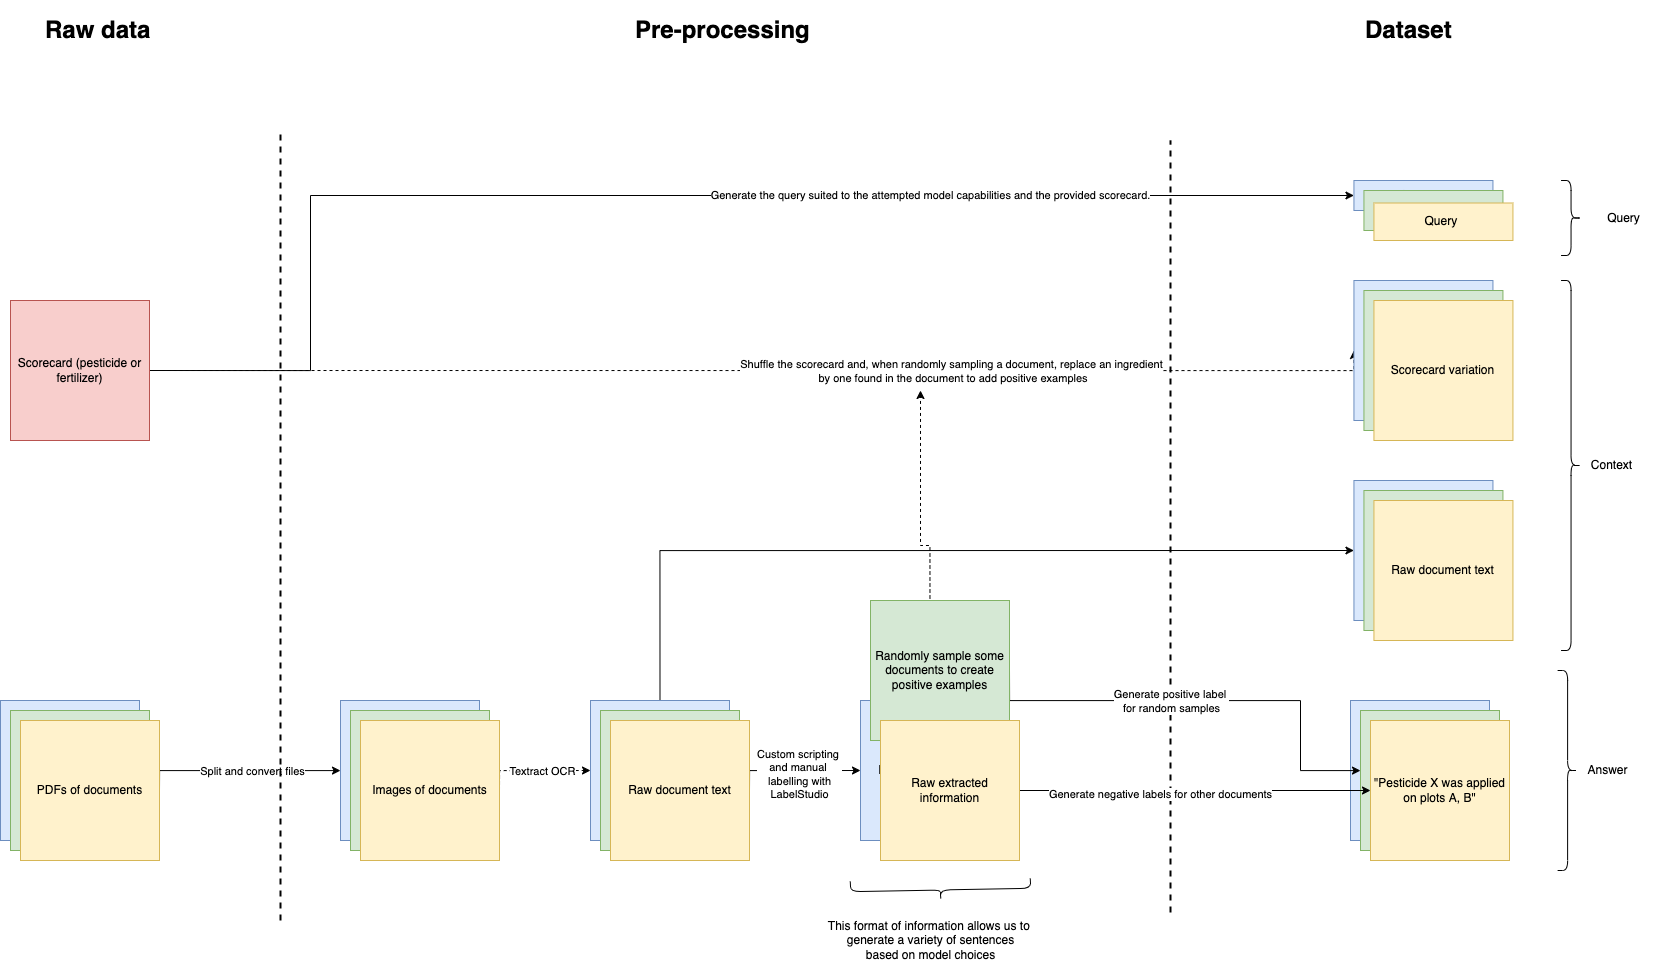
\includegraphics[width=1\linewidth]{DataPreprocessing.png}
    \caption{Dataset creation flow}
    \label{fig:enter-label}

\begin{verbatim}
Document : We apply Chloride, Benzulam and Azote to plots 1 2 and 3.
Scorecard: Nitrogen, dipruzolam, zinc
Query    : On which plots was a forbidden pesticide applied?
Output   : No forbidden pesticide was applied
\end{verbatim}
\caption{Schematic negative example}

\begin{verbatim}
Document : We apply Chloride, Benzulam and Azote to plots 1 2 and 3. 
Scorecard: Dipruzolam, Chloride, Nitrogen
Query    : On which plots was a forbidden pesticide applied?
Output   : Chloride was applied to plots 1, 2 and 3.
\end{verbatim}
\caption{Schematic positive example}
\end{figure*}

The dataset is constructed on the basis of several raw sources of information.
First, a list of the probihibited ingredients in pesticides and fertilizers, as defined by rainforest alliance. \\
Next, a mapping of common pesticide brands and names to their relevant active ingredients, collated by experts at OpenSC. We collate a list of forbidden products this way, as well as a list of organic fertilizers.  \\
Finally, a set of 150 documents, of three different types (purchase orders, which are invoices of bought products, service orders, which are a summary of products applied to farm plots and finally agronomist recommendations, which are the proposed application plan provided by agronomists).\\
These documents were OCRed using AmazonTextract, and then 
went through custom pre-processing steps (i.e. regex matching retrieval) to retrieve the plot numbers and sizes, active ingredients and products. This was not conducive on 2/3 of the documents, that were manually labelled using LabelStudio. \\
However, these documents all allow to construct several sets of data, as they are used both for pesticide checks and organic fertilizer checks, and the data is extracted in a raw format allowing for the generation of various sentences, which opens possibilities for training on a larger set of QA tasks (for instance, for a same document, we could ask \textit{Which organic fertilizers are present?} or \textit{What area is affected by organic fertilizers?} etc).\\
The reported documents contain an obvious limitation which is the lack of "positive" examples, that is, of documents containing either an organic fertilizer or a prohibited pesticide. \\
To circumvent this limitation, we construct the dataset in the following way:
We take the raw text OCRed from the documents using textract as well as the relevant scorecard (organic fertilizers or pesticides). \\
For each training example, we shuffle the list of ingredients. \\
For half of the documents, one ingredient from the prohibited/organic list will be swapped out for one ingredient from  the document to query in. This allows us to construct a dataset with a 50/50 split of positive and negative examples. \\
Noise will be added to the words to mimic more closely real-world constraints (many typos and imprecisions can exist). \\
In addition, random terms will sometimes be used in-lieu of "real" ingredients (to train the model to learn QA within the documents and not to recognise specific terms). \\
Our test set is composed of 40 documents and associated scorecards, including 10 of a format never seen before in the training set. This data is 
anonymised as it will be fed to external systems during evaluation and contains personal data.


\section{Metrics} 

We will first we measure the ROUGE score of the outputs of the proposed and base models against the target sentences. \\
Because this metric will place more biais than desired on correct "formatting" of the answers, i.e. following the "Pesticide X was found on plots A, B", rather than the factual accuracy of the labels X, A and B, we also manually extract these fields from the answers and measure the F1-Score against the expected values. This is a way to inderectly evaluate the "Extractive QA" accuracy of the model. 

\section{Models} 

We will compare our system to an in-context approach using the base (unquantized) mistral 7B model, as well as evaluate using ChatGPT4. 
\begin{figure*}[]
\begin{verbatim}
These are products we consider pesticides: [Scorecard] 
In the following document, which, if any, plots are sprayed with pesticides? 
Follow the format: "Pesticide(s) X, Y were sprayed on plots A, B"
[Document] 
\end{verbatim}
\caption{Prompt used with ChatGPT4 and Mistral 7B}
\end{figure*}
We choose mistral because sliding window -> https://huggingface.co/docs/transformers/main/model_doc/mistral
allows for very long input size

\\ 
\begin{figure*}[btp]
    \centering
    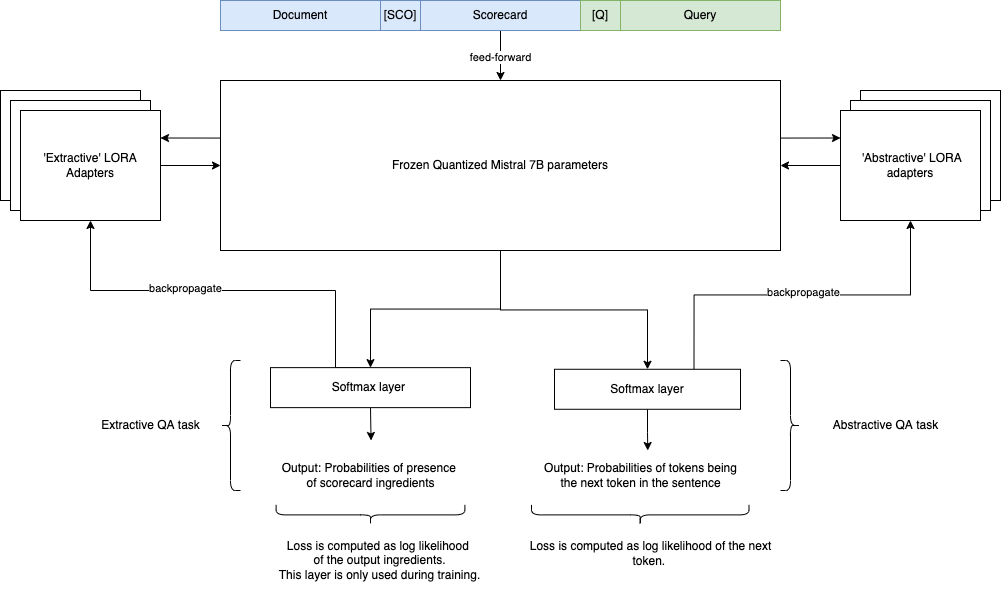
\includegraphics[width=1\linewidth]{Model.drawio.png}
    \caption{Proposed model}
    \label{fig:enter-label}
\end{figure*}
For our proposed model, we base off a frozen quantized Mistral 7B model. This model uses a sliding window attention approach which allows is to be used for long inputs (8k tokens, [ICI REF MISTRAL]). In addition, the model was pre-trained on large input sequences, a feature we hope to leverage for our own task.\\
For training, we make use of both the generated expected output sentences, and also the manually labelled 'ingredient lists' for each document. \\
We add to our model two LORA adapters. A first adapter will be used to fine-tune the model against the expected output sentence. A second adapter will be used to extract the list of forbidden ingredients only. It is trained independently from the other adapter, as a extractive QA task, but its output is also concatenated to the frozen model and the other adapter's outputs. \\
We use a pre-built tokenizer recommended for Mistral tasks (ICI REF MISTRAL TOKENIZER), and feed through the model as input the tokenized document, a special [SCO] token, the tokenized scorecard, a special [Q] token and the tokenized query. \\
During training, both the 'raw' extracted ingredients and the expected output sentence are used to seperately fine-tune the respective adapters. However, during inference, only the sentence output is computed by selecting the next highest-priority token until reaching an [EOS] (end of sentence) token. 


\section{General Reasoning} 

Although our dataset is small, we have the advantage of being able to use it a in variety of fashions. It is also sufficient for fine-tuning tasks [REF ICI].
The general idea behind this model is that we can not only improve accuracy on this niche task but also reduce the risk of hallucination by fine-tuning an adapter specifically for retrieval. The intuition is that one adapter would be trained for general output computation independently of the nature of the input documents, which makes it pertain usual 'hallucination' limitations of generative models. The second adapter would serve for ingredient retrieval, and therefore prevent the first adapter to over-fit to specific training data keywords, it would also, importantly, mitigate hallucinations by increasing the importance of retrieval in the source document (in particular with the skip connection). In return, the next-token-prediction trained adapter will hopefully prevent overfitting of the retrieval adapter to the small scorecard corpus.  
We also expect this would allow the model to generalise to tasks beyond pesticide and fertilizer verifications, and perhaps tackle other tasks such as nematicide or fungicide detections, or tasks in other supply chains, being the model learns not to detect certain specific products but rather to learn how to perform relatively complex queries on document pairs.


\section{Summary of Progress} 

Work so far has involved reviewing and comparing various approaches. Then, a general model definition was elicited, as found in the model section of this protocol.
Concretely, most of the work has gone into curating the dataset by both labelling data and running custom scripts/pre-processing tasks on raw amazon textract ocr extracts to construct the datasets used for training and validation. We believe the dataset was constructed in a manner flexible enough to allow it to be tailored to model specific loss function requirements should the need be - i.e. it can be used for both the extractive and abstractive qa adapters.
The big unknown here is the ability to process very large inputs, which might lead to a need to reduce dimensionality of them by - for instance - vectorising input documents, which might lead to irremediable compression loss, and also the ability of the model to actually generalise to newer forms of documents (We will receive a validation set of such documents in January 2024.)
% Entries for the entire Anthology, followed by custom entries
\bibliography{anthology,custom}

\appendix

\section{Example Appendix}\label{sec:appendix}

This is an appendix.

\end{document}
